\section{Solution Methods for Elliptic Partial Differential Equations}
\label{sec:solution-methods-for-elliptic-pdes}

The discretization methods described in \refsec{sec:numerical-methods-for-elliptic-pdes} result in a linear system. To generally talk about these solution methods, we assume that we form the linear system
\begin{align}
    \textbf{A} \textbf{u} = \textbf{b}
    \label{eq:ls}
\end{align}
where $\textbf{A} \in \mathbb{R}^{N \times N}$ is a coefficient matrix formed from one of the discretization methods, $N$ is the number of degrees of freedom, $\textbf{u} = u_i = u(x_i)$ for $i \in \textbf{I}_x$, index set $\textbf{I}_x$ for the discrete domain, and $\textbf{b}$ is the right-hand side vector encoded with the boundary conditions and the inhomogeneous function $f(\textbf{x})$. The goal is to solve for $\textbf{u}$ where we take advantage of the sparsity and structure of $\textbf{A}$. We organize the various methods into the following three categories: 1) iterative methods, 2) direct methods, and 3) hierarchical methods.

\subsection{Iterative Methods}
\label{sub:iterative-methods}

Iterative methods start with an initial guess of a solution to \ref{eq:ls} and correct the iterate until convergence to a specified tolerance. The simplest iterative methods are called splitting methods where the linear system is modified according to
\begin{align}
\textbf{A} = \textbf{M} - \textbf{N} \Rightarrow \textbf{M} \textbf{u} = \textbf{N} \textbf{u} + \textbf{b}.
\end{align}
This suggests the following recursion relationship for the next iteration:
\begin{align}
\textbf{M} \textbf{u}^{k+1} &= \textbf{N} \textbf{u}^k + \textbf{b} \\
\textbf{u}^{k+1} &= \textbf{M}^{-1} \textbf{N} \textbf{u}^k + \textbf{M}^{-1} \textbf{b}.
\end{align}
The idea is to choose $\textbf{M}$ that captures as much of $\textbf{A}$ as possible, but is still easy and quick to invert. As $\textbf{A}$ is either banded or sparse, classical splitting methods for elliptic PDEs split $\textbf{A}$ into $\textbf{A} = \textbf{D} - \textbf{L} - \textbf{U}$, where $\textbf{D}$ is the diagonal components of $\textbf{A}$, and $\textbf{L}$ and $\textbf{U}$ are the lower and upper pieces, respectively. Classical choices for $\textbf{M}$ and $\textbf{N}$ are summarized in Table \ref{tab:splitting}.

\begin{table}[h!]
    \centering
    \begin{tabular}{ | l | l | l |}
        \hline
        Jacobi & $\textbf{M} = \textbf{D}$ & $\textbf{N} = \textbf{L} + \textbf{U}$ \\
        Gauss-Sidel & $\textbf{M} = \textbf{D} - \textbf{L}$ & $\textbf{N} = \textbf{U}$ \\
        Successive Over Relaxation & $\textbf{M} = \frac{1}{\omega}(\textbf{D} - \omega \textbf{L})$ & $\textbf{N} = \frac{1}{\omega} \big( (1 - \omega) \textbf{D} + \omega \textbf{U} \big)$ \\
        \hline
    \end{tabular}
    \caption{Iterative Methods: Splitting Methods}
    \label{tab:splitting}
\end{table}

Another class of iterative methods are called Krylov subspace methods. The Krylov space is defined as
\begin{align}
\mathcal{K}_k = \text{span} \{ \textbf{r}_0, \textbf{A} \textbf{r}_0, \textbf{A}^2 \textbf{r}_0, ..., \textbf{A}^{k-1} \textbf{r}_0 \}
\end{align}
based on the initial residual $\textbf{r}_0 = \textbf{b} - \textbf{A} \textbf{u}^{(0)}$. The goal is to take the next iteration from this particular space. Two common Krylov methods are the Conjugate Gradient method \cite{hestenes1952methods} and the Generalized Minimal Residual (GMRES) method \cite{saad1986gmres}. In the conjugate gradient method, the approximation is adjusted by a conjugate direction, or a vector that is conjugate with respect to $\textbf{A}$. This vector is called the search direction $\textbf{p}$ and is scaled by $\alpha$, which is computed by solving a quadratic minimization problem. The GMRES method builds up an orthogonal matrix $\textbf{Q}$ through a process called the Arnoldi iteration. The Arnoldi iteration forms $\textbf{A} = \textbf{Q} \textbf{H} \textbf{Q}^*$ for orthogonal matrix $\textbf{Q}$ and Hessenberg matrix $\textbf{H}$. The next iteration is found via $\textbf{Q} \textbf{y}$ where $\textbf{y}$ is found from a least squares problem involving $\textbf{H}$. These methods are summarized in Table \ref{tab:ksm}.

\begin{table}[h!]
    \centering
    \begin{tabular}{ | l | l |}
        \hline
        Conjugate Gradient & $\textbf{u}^{(k+1)} = \textbf{u}^{(k)} + \alpha^{(k)} \textbf{p}^{(k)}$ \\
        GMRES & $\textbf{u}^{(k)} = \textbf{Q}^{(k)} \textbf{y}$ \\
        \hline
    \end{tabular}
    \caption{Iterative Methods: Krylov Subspace Methods}
    \label{tab:ksm}
\end{table}

Most iterative methods are considered ``matrix-free" methods. A ``matrix-free" method is a method that does not explicitly form the matrix $\textbf{A}$, but is rather applied to a vector. For example, if implementing a Conjugate Gradient method for a finite difference discretization, one has to compute the product $\textbf{A} \textbf{u}^{(k)}$. Instead of doing the full matrix-vector calculation, one can write a function that takes $\textbf{u}$ and returns the 2nd-order, central difference operator as computed in \ref{eq:poisson_FD}.

As finite difference discretization schemes for elliptic PDEs lead to sparse matrices, the application of $\textbf{A}$ to a vector can be done in $\mathcal{O}(N)$ operations, where $N$ is the number of unknowns in the vector. Thus, the performance for most iterative methods is approximately $\mathcal{O}(N \times N_{iter})$, where $N_{iter}$ is the number of iterations required for a specified tolerance. However, as $N$ gets larger, often so does $N_{iter}$, leading to poor scaling, as noted in \cite{martinsson2019fast}. In addition, iterative methods may not always converge for a given initial guess or structure of $\textbf{A}$, which make them unfavorable for ``black-box" implementations for linear solvers.

\subsection{Direct Methods}
\label{sub:direct-methods}

Motivation for direct solvers stems from wanting to improve upon the disadvantages of iterative methods. Martinsson notes in \cite{martinsson2004fast} some advantages to using direct methods over iterative ones:
\begin{itemize}
    \item Direct methods can be applied to multiple right-hand side vectors $\textbf{b}$ or multiple boundary conditions once a factorization or solution operator is built, whereas iterative methods must be solved anew for each right-hand side or for different boundary conditions.

    \item Direct methods can take advantage of ``close" matrices (i.e. if we have an inverse or factorization of $\textbf{A}$ and perturb it by $\epsilon$, we could adjust the inverse to account for it instead of recompute the inverse).

    \item Most direct methods can take advantage of fast and efficient algorithms for matrix factorization such as the singular value decomposition, LU decomposition, QR decomposition, etc.
\end{itemize}
We will look at how direct methods are useful as we consider some common direct methods from \cite{leveque2007finite} and \cite{trefethen1997numerical}.

Many direct methods are based on matrix factorizations. Perhaps the most well-known is the LU decomposition. LU decomposition factors the coefficient matrix into a lower and upper triangular matrix: $\textbf{A} = \textbf{L} \textbf{U}$. The idea is to use Gaussian elimination to eliminate entries below the main diagonal, and then use back-substitution to solve for each entry in $\textbf{u}$. In general, LU decomposition requires $\mathcal{O}(N^3)$ floating point operations and thus is impractical for large matrices. There are banded solvers for Gaussian elimination that can take advantage of the sparsity of a matrix. The Cholesky decomposition is a variant of Gaussian elimination for symmetric matrices. Other matrix factorizations include the QR-decomposition, $\textbf{A} = \textbf{Q} \textbf{R}$, and the singular value decomposition, $\textbf{A} = \textbf{U} \boldsymbol{\Sigma} \textbf{V}^*$.

For a finite difference discretization of elliptic PDEs, $\textbf{A}$ is banded and sparse, and more efficient algorithms for LU decomposition exist. For 1D problems, $\textbf{A}$ is diagonally dominant and sparse with the bandwidth (the number of entries off the main diagonal in a matrix) dependent on the order of the stencil. For the stencil shown in the second order discretization in \ref{eq:poisson_FD}, $\textbf{A}$ is tridiagonal. This allows us to use algorithms such as Thomas's algorithm for solving a tridiagonal system in $\mathcal{O}(N)$ steps (\cite{higham2002accuracy}). In higher dimensions, block versions of Thomas's algorithm exist (\cite{quarteroni2010numerical}).

Compared to iterative methods, direct methods will terminate in a finite number of steps. Direct methods are more fit for ``black-box" implementations. However, because most direct methods need to explicitly form $\textbf{A}$, they are more difficult to implement with limited computing resources. Indeed, going to higher dimensions and higher orders often dramatically increases memory and compute requirements.

\subsection{Hierarchical Methods}
\label{sub:hierarchical-methods}

The methods grouped under hierarchical methods attempt to accelerate some of the ideas from iterative and direct methods by breaking the problem into a hierarchy of subproblems. By recursively breaking the original problem into smaller subproblems, significant improvements can be made in complexity and performance. We'll talk about three hierarchical methods here: the multigrid method, nested dissection, and the Hierarchical Poincaré-Steklov (HPS) method.

\subsubsection{The Multigrid Method}
\label{subsub:multigrid-method}

The multigrid method was introduced by Brandt in \cite{brandt1977multi}. It has been widely used in various applications and for all types of solution methods. Briggs in \cite{briggs2000multigrid} gives an overview and tutorial of the multigrid method.

In the multigrid method, the idea is to use multiple levels of grids and solution methods on each level to solve a larger problem. To look at the multigrid method, we define the error in the linear system to be $\textbf{e} = \textbf{u}^{(k)} - \textbf{u}_{exact}$ (the difference between the exact solution and the $kth$ iteration). After a few iterations of a smoother (typically Jacobi's method), because of the local averaging, any high-frequency error is quickly dampened away. What takes longer to eliminate is the low-frequency error associated with the global problem. By coarsening the grid, the lower frequency error is dampened quicker. Multigrid combines the ability of iterative methods to locally reduce error and a coarsening grid technique to accelerate convergence.

In the multigrid method, one starts with the solution on a fine grid, for example, with grid spacing $h$, and performs a few iterations of a smoother. After a few iterations, the $h$-level grid is projected onto a coarser $2h$-level grid. On this level, one performs a few more iterations of a smoother. Because the grid is coarser, this step is faster. Again, after a few iterations, the solution is projected onto an even coarser $4h$-level grid and a few more iterations are performed. This is done a specified number of times, and then the solution is interpolated back up the levels to the original grid. This is shown in Figure \ref{fig:multigrid}.

\begin{figure}
    \centering
    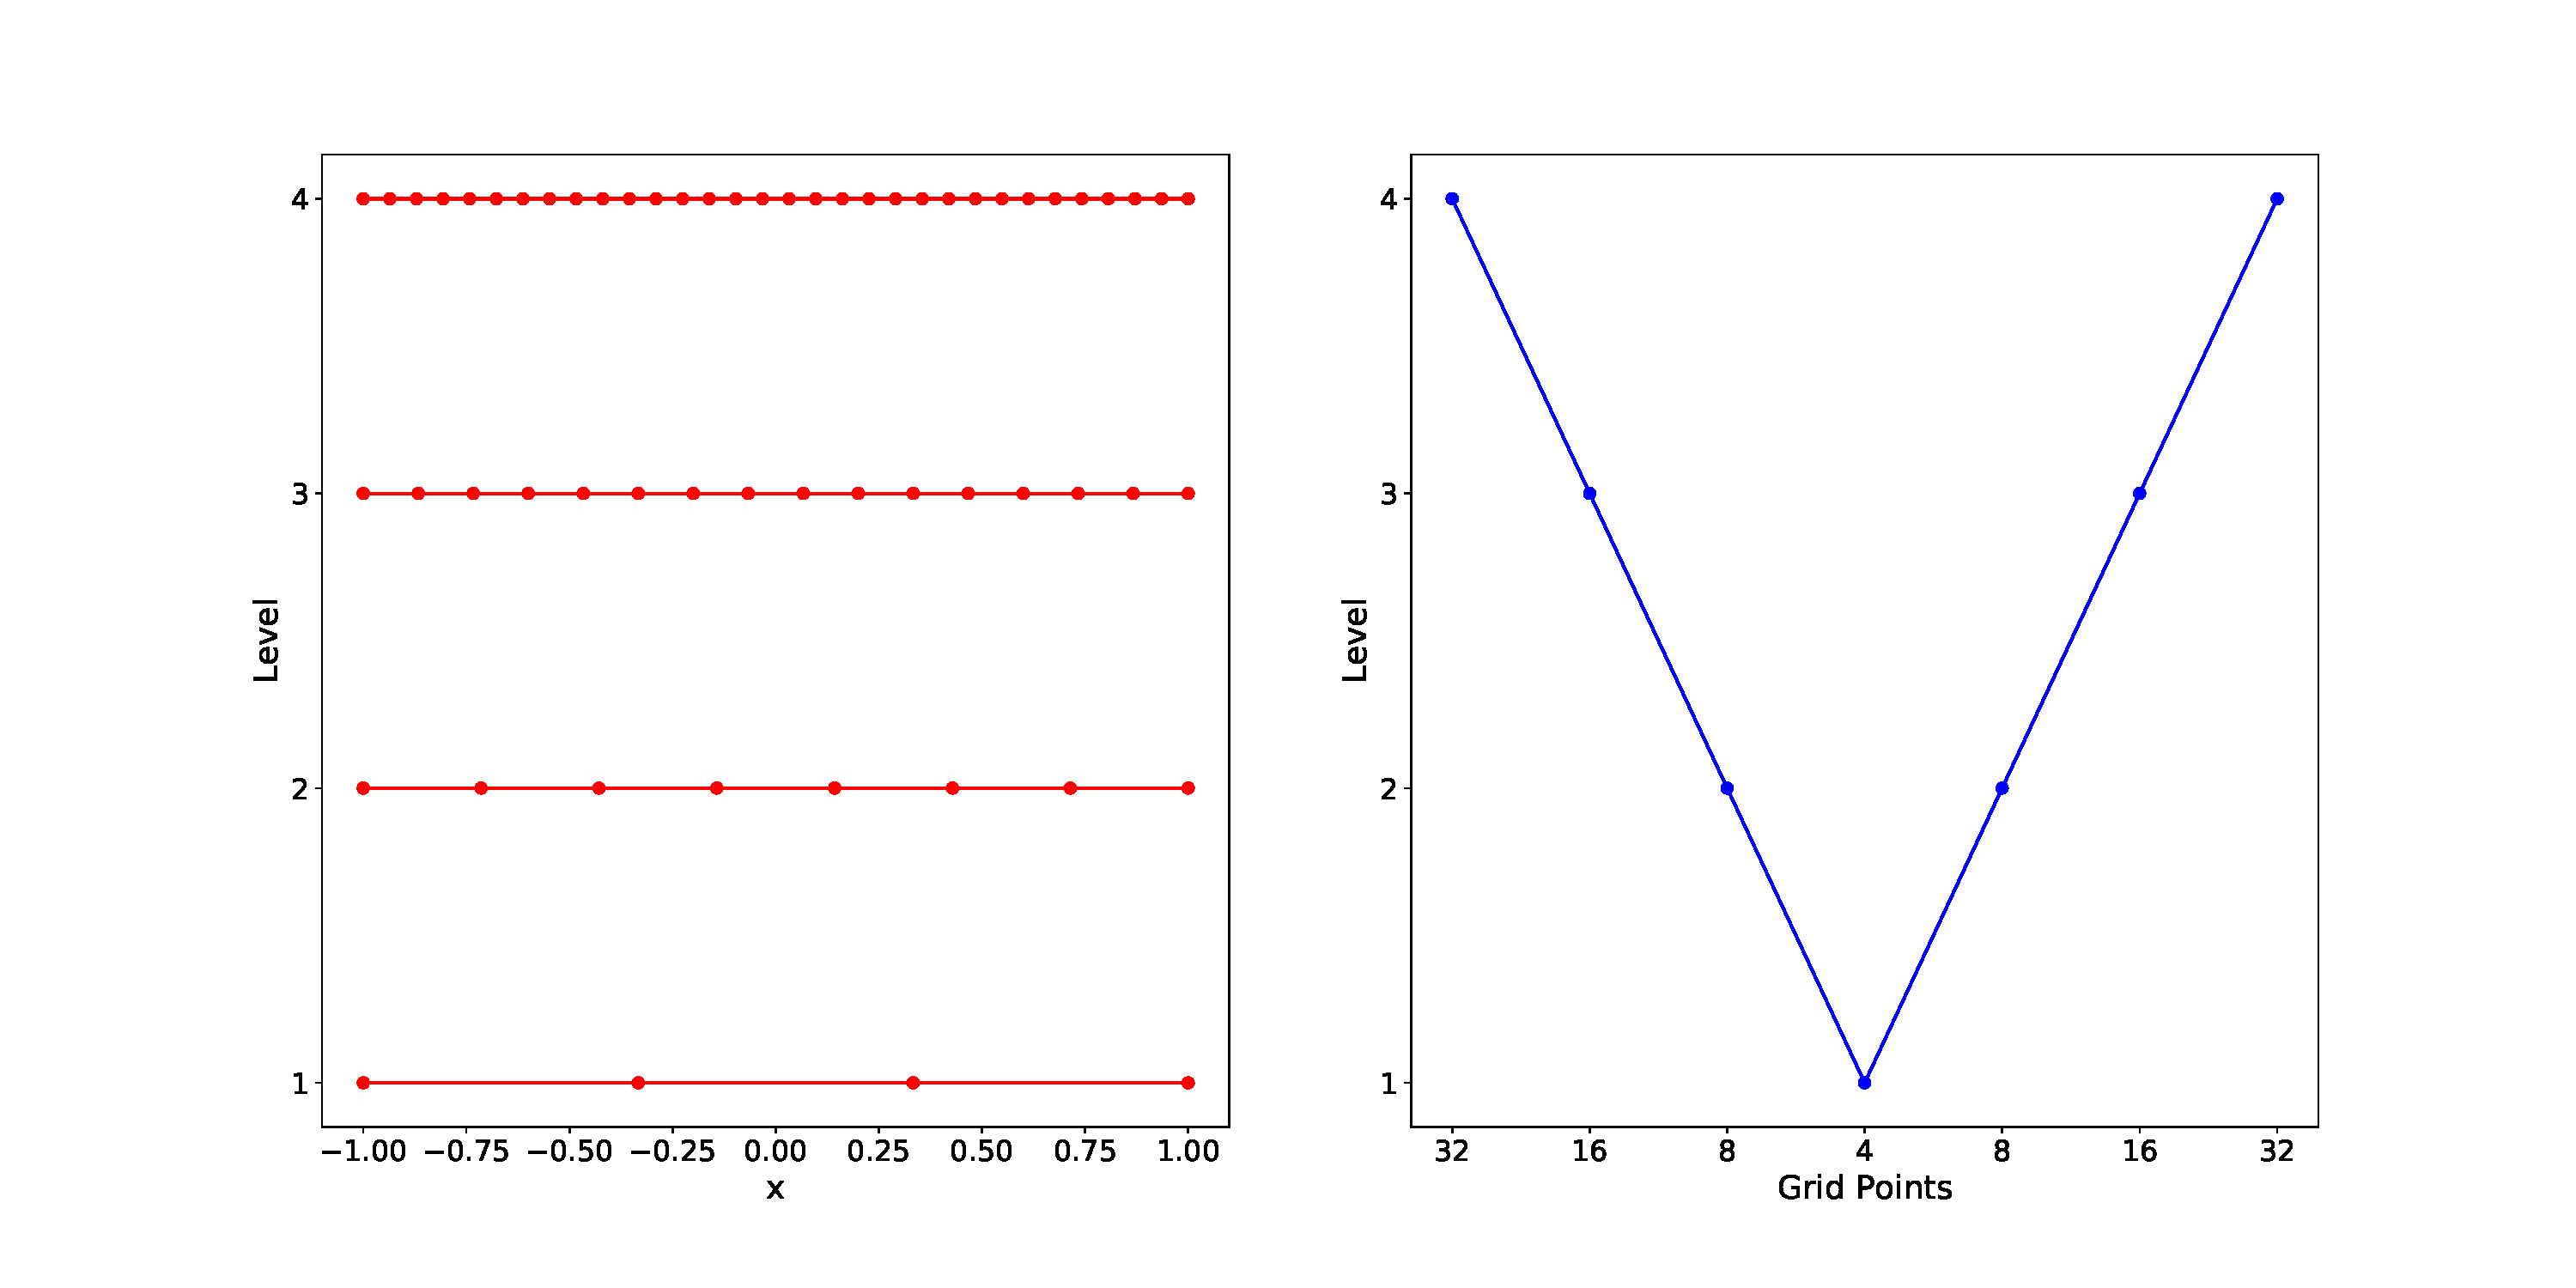
\includegraphics[width=0.8\columnwidth]{figures/multigrid.pdf}
    \caption{The 1D Multigrid Method. Starting with the finest grid, perform a few iterations of an iterative method. This is called relaxing the solution. Then project onto a coarser grid, and relax again. Do this down the levels in the grid to a desired precision. Once the solution is converged to on the coarsest level, interpolate back up the levels to obtain the solution on the finest level.}
    \label{fig:multigrid}
\end{figure}

In what is called the ``full multigrid" method, the process starts on the coarsest level instead of the finest. The solution is relaxed on this level, and then interpolated down onto a finer mesh. The interpolated solution is used as an initial guess for solving the problem on the finer mesh. The relaxed solution on a coarser grid is often an ideal initial guess for the problem on the finer mesh, resulting in quick convergence on that level.

The multigrid method allows one to accelerate an iterative solver. Multigrid methods are very effective as pre-conditioners for iterative methods. This is the general pattern of hierarchical methods: the ability to use classical iterative and direct methods on smaller grids where they perform well, and then ``scale" them up to larger problem sizes.

\subsubsection{Nested Dissection}
\label{subsub:nested-dissection}

The nested dissection method formulated by George in \cite{george1973nested} is a direct method that builds upon Gaussian elimination for problems on a grid. It is also the basis for forming what is called the multifrontal method. By taking advantage of the ordering of points on a grid, one can permute $\textbf{A}$ to first eliminate points that split the mesh into two unconnected meshes. This permutation takes the form of $\textbf{P}^* \textbf{A} \textbf{P}$, where the goal is to form $\textbf{P}$ to reorganize $\textbf{A}$ in a way that eliminates points in an efficient manner.

To detail nested dissection better, consider an $N \times N$ mesh such as a finite difference mesh discussed in Section \ref{sec:elliptic}. Assume that the initial ordering of points corresponds to an index set that iterates over the points in the mesh row-by-row. Now, the idea of nested dissection is to reorganize the points such that we first eliminate points down the middle of the mesh (i.e. the points at $x = 0$ in the first plot of Figure \ref{fig:discretization_methods}). Once these points are solved for, it spilts the mesh into two equally sized pieces that are disconnected. Each of the disconnected meshes now are smaller, and thus easier to solve. This idea of splitting the mesh into disconnected pieces by first eliminating points along an interface can be recursively applied to each split. This means that after dividing the mesh into two, one can divide those two meshes into four meshes, and so on. Recursive splitting is a common characteristic in hierarchical methods.

Nested dissection was first introduced by George in \cite{george1973nested}, and further generalized by Lipton et al. in \cite{lipton1979generalized}. Martinsson has a tutorial on nested dissection in \cite{martinsson2019fast}. In fact, nested dissection served as motivation for another hierarchical method proposed by Martinsson and Gillman called the Hierarchical Poincaré-Steklov method.

\subsubsection{The Hierarchical Poincaré-Steklov Method}
\label{subsub:hps-method}

The work done by Gillman and Martinsson in \cite{martinsson2004fast}, \cite{MARTINSSON2013460}, and \cite{gillman2014direct} (with a practical tutorial found in \cite{martinsson2015hierarchical}) culminate in what they call the Hierarchical Poincaré-Steklov (HPS) method. It is a direct solver for elliptic PDEs that is based on a binary tree of rectangular patches where the solution operator to $\textbf{A}$ is built by recursively merging child patches. Like direct methods, the HPS method involves a factorization step and a solve step. The chief advantage of the HPS method over other direct methods is that it does not require the explicit formulation and storage of $\textbf{A}$.

The HPS method starts with an original problem domain, and recursively divides the domain in half. This creates a binary tree of patches as shown in Figure \ref{fig:solve}. Once the domain has been decomposed into this tree of patches, two operators are defined on the lowest level, called the leaf level. These operators are the solution operator $\textbf{S}$ and Dirichlet-to-Neumann (DtN) operator $\textbf{T}$. The solution operator maps boundary data to solution data on the interior of the patch (i.e. solves the local boundary value problem), and the DtN operator maps Dirichlet data on the boundary to Neumann data on the boundary. These operators can be formed using any elliptic PDE solver, including fast solvers like spectral methods. After forming these operators, the next step is to recursively merge each sibling patch up the tree. the merge step is demonstrated in Figure \ref{fig:merge}. This results in a global solution operator that can be stored and used multiple times (at different time steps or with varying boundary conditions, etc.), and is similar to a direct method matrix factorization. The final step is applying the solution operator to each level down the tree to obtain the solution everywhere in the domain. This step is just a matrix-vector multiplication and is very fast.

Similar to other direct methods, the HPS method forms an in-memory solution operator that can be applied to several right-hand side vectors. This property makes it ideal for problems where several elliptic solves are necessary. While most iterative methods have better asymptotic performance than other direct methods, the HPS method can be accelerated using hierarchically block seperable (HBS) matrix algebra to achieve near linear asymptotic performance (\cite{gillman2014direct}).

\begin{figure}
    \centering
    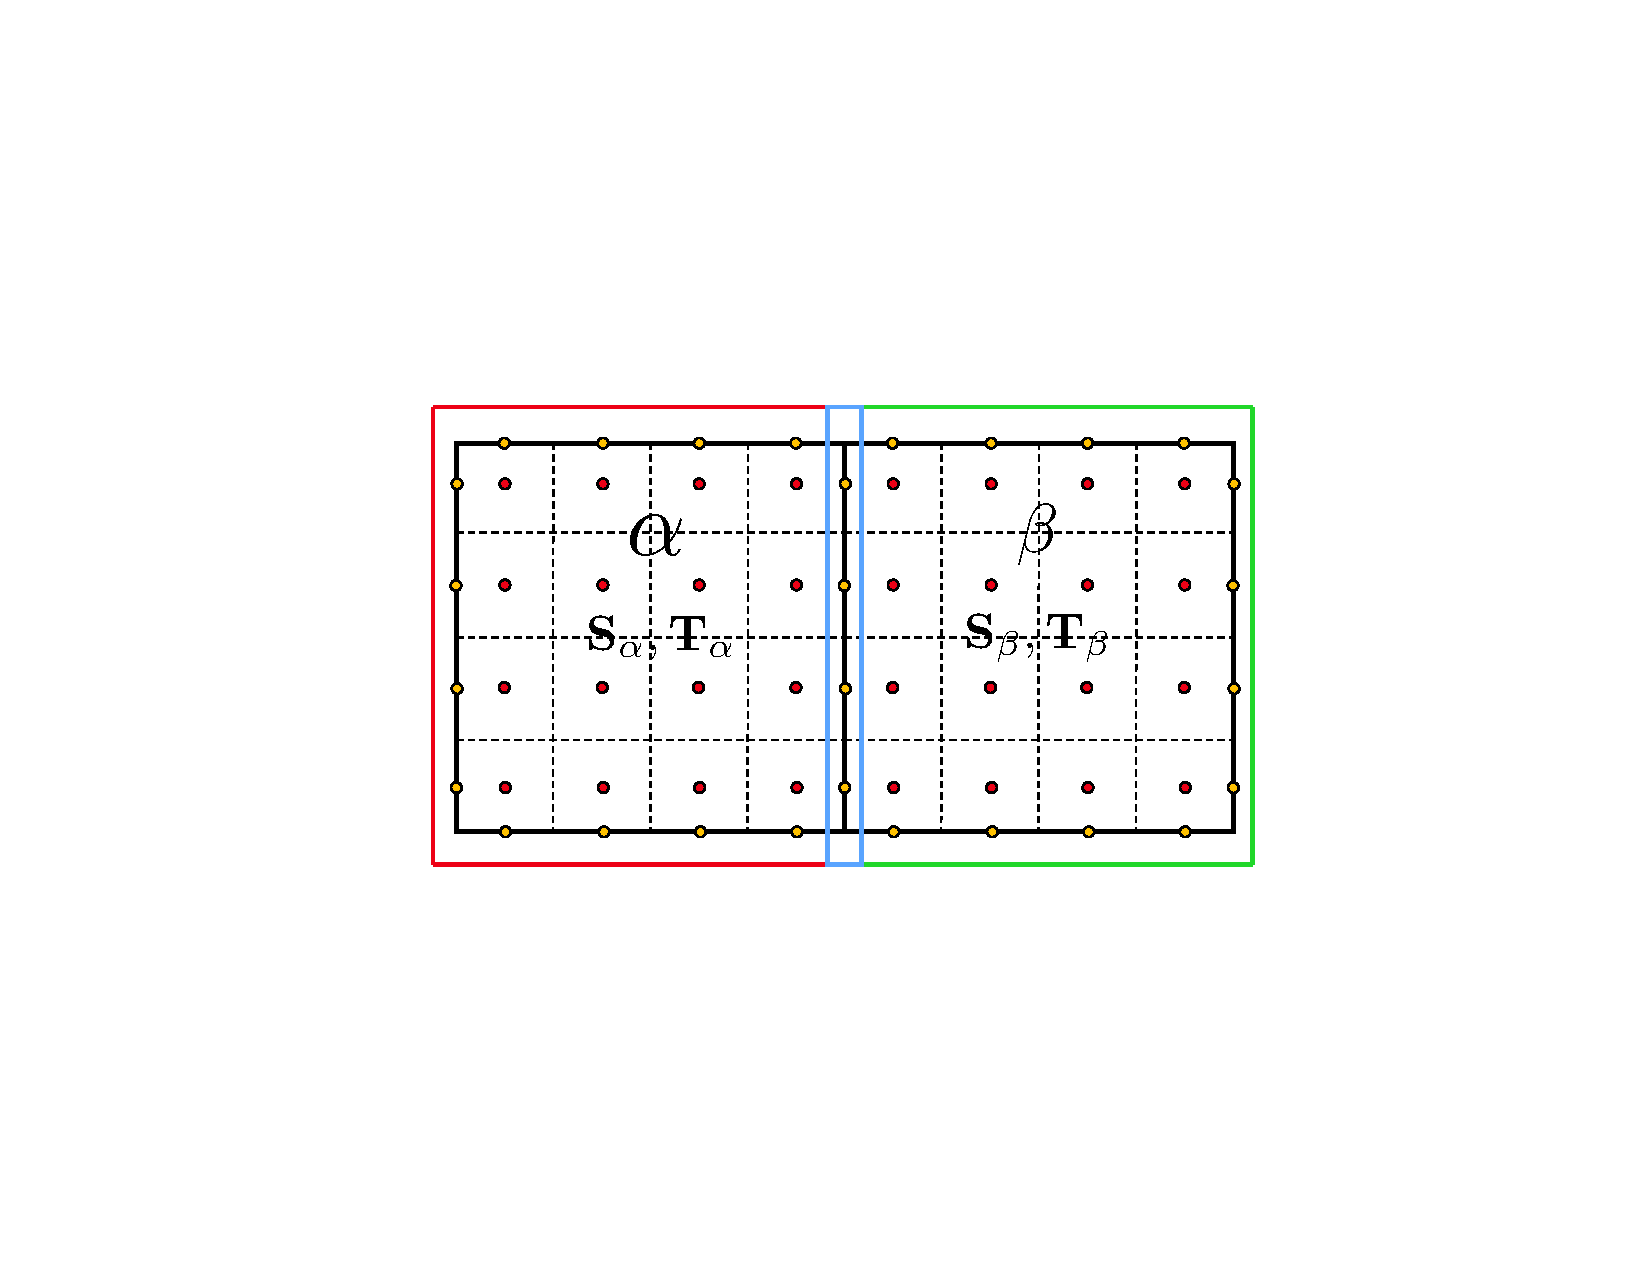
\includegraphics[width=0.7\columnwidth]{figures/merge_figure.pdf}
    \caption{HPS Merge Operation. The merged patch $\Omega_{\tau}$ is the union of children $\Omega_{\alpha}$ and $\Omega_{\beta}$, i.e. $\Omega_{\tau} = \Omega_{\alpha} \cup \Omega_{\beta}$. Red, green, and blue nodes correspond to index sets $\textbf{I}_1$, $\textbf{I}_2$, and $\textbf{I}_3$, respectively. The merge operation eliminates the nodes on the interface of the children patches.}
    \label{fig:merge}
\end{figure}

\begin{figure}
    \centering
    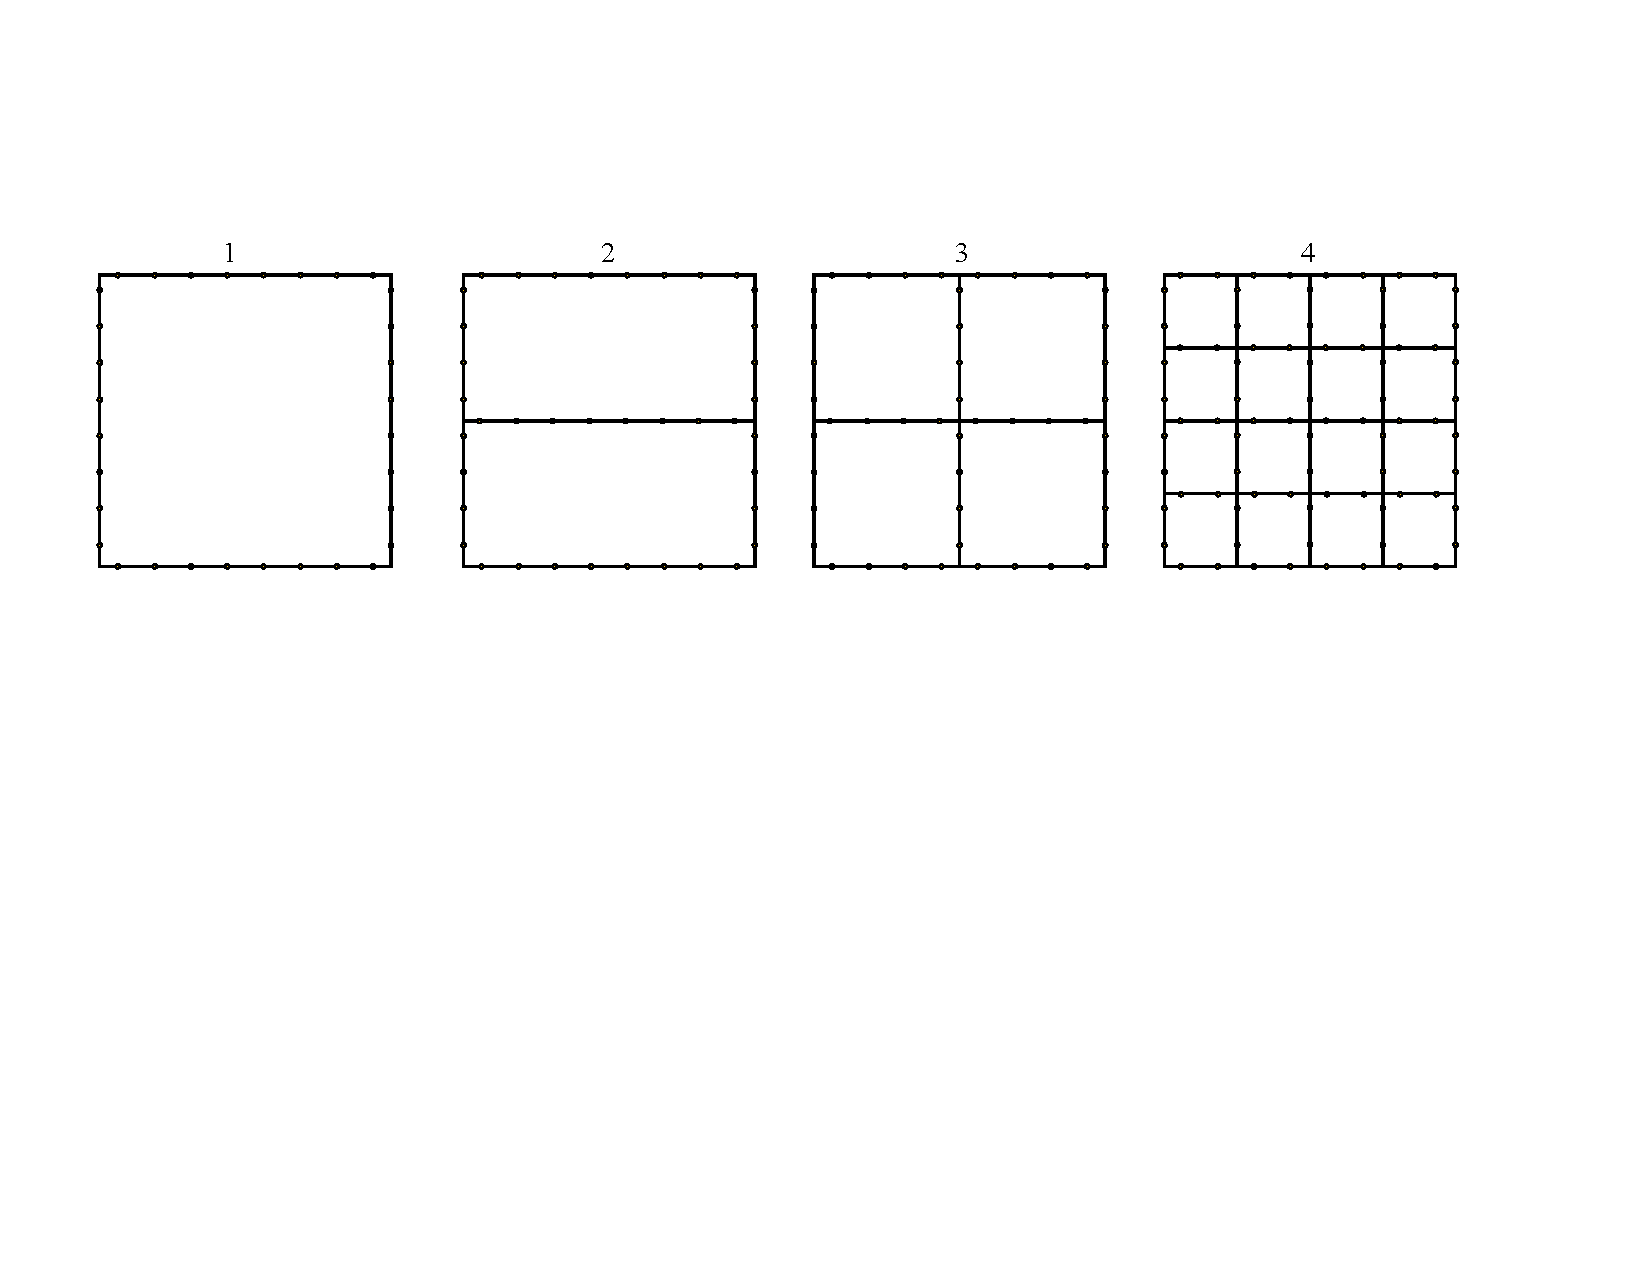
\includegraphics[width=\columnwidth]{figures/solve_figure.pdf}
    \caption{HPS Solve Stage. Once $\textbf{S}_0$ is formed, apply it to the top level Dirichlet data to get boundary (and solution) data on the interface of the children. Apply the patch solution operator down the tree until each leaf has it's local boundary information. Then apply the solution operator to get the solution data in the interior of each leaf.}
    \label{fig:solve}
\end{figure}
